\documentclass[a4paper,10pt]{article}
\usepackage{graphicx}
\usepackage[utf8]{inputenc}

%opening
\title{ViewMind Software Suite}
\author{Ariel E. Arelovich}

\begin{document}

\maketitle

\section{Introduction}

This manual is intented to document and describe the ViewMind Software Suite with enough detail to enable modification of its sourcode. A good understanding of the Qt libraries is absoluetly fundamental for understanding the source code. In particular, the Qt Signal-Slot system, the QML/QtQuick framework for developing advanced UI, the QtNetwork framework for establishing TCP connections and the QSql framework for working with MySQL databaseses.


\section{Overview}

The ViewMind software suite is composed, mainly, of three components: The EyeExperimenter (the client application), the EyeServer (Manages communication with the server side software, as well as communication with the database) and the EyeReportGenerator. The interections between these programs can be seen in Figure~\ref{fig_overview}.

\begin{figure}[!h]
\centering
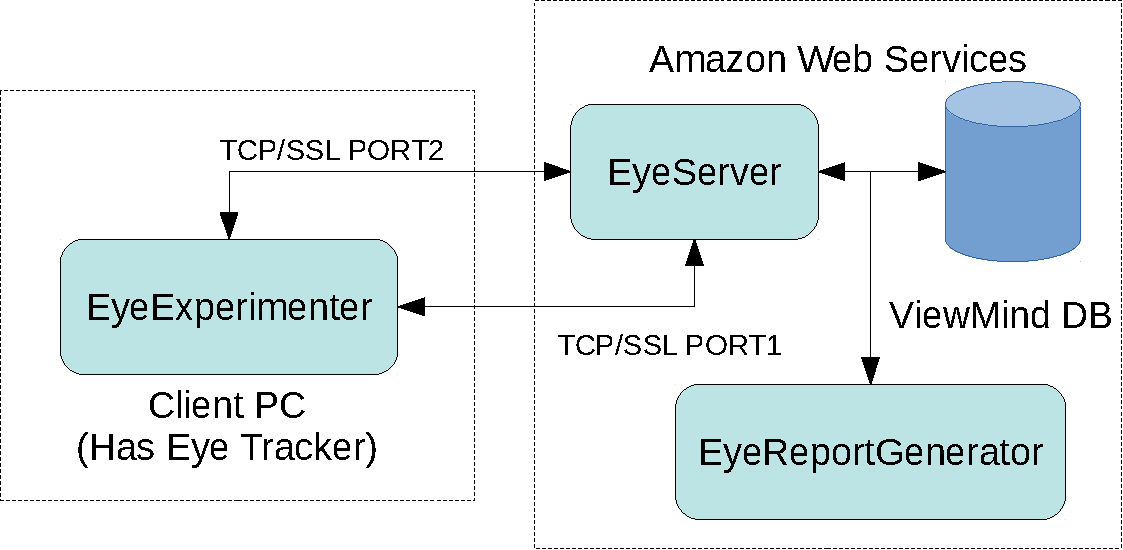
\includegraphics[scale = 0.5]{overview-crop.pdf}
\caption{Main components of the ViewMind Software Suite and its interactions}
\label{fig_overview}
\end{figure}

The software was designed to run in the following manner. The EyeExperimenter is the main application. It need to run on Windows PC, connected to the EyeTracker (and the EyeTracker software). The EyeTracker Software (which depends on the EyeTracker beign used) needs to be running before starting the EyeExperimenter itself. 

The EyeExperimenter allows the configuration of the Doctor information, and the registration of new patients. This when this happens it uses opens up an encrypted connection to the server (using the OpenSSL libraries for managing this encrypted connection) and sends the data to be stored in the Database. It can also request data for a patient or doctor given the person's unique ID. At the time of this document the port used for the DB connections is 54915. The EyeServer receives these requests and transforms them into proper queries to the Viewmind DB returning the results, if necessary, to the EyeExperimenter. It is important to note that each connection is atomized. That is, a connection is opened to the EyeServer each time data is required and then close after the data is sent (or received) in each instance. This avoids the problem of establishing a connection that falls during, say, the middle of an study.

The configuration of the EyeExperimenter allows the selection of a Demo Mode, the use of Second Monitor and, most important, the selection of the EyeTracker to use. It also allows the selection of the output directory. This variables is very important as once it is selected all file and directory generation required the the EyeExperimenter is automatized. 

%(in which only the first three trials of a given test are executed and the data sent to server is preloaded in the program)

Once the patient and doctor information is sorted and the EyeTracker was selected, the studies can begin. The selected tests will be run one after the other with a screen providing a short description of each test to the patient. The data will be saved in predefined directories (See Directory Structure).

Once the tests have concluded, a processing request is sent to the EyeServer using a different port (54915). The EyeSever receives the processing requests and sends another request fo the data to be processed when one of its processing slots is free. This is configurable and limits the number of parallel instances fo the EyeReportGenerator than will run in the server. 

When the EyeExperimenter receives the request for data, it sends the newest file for each study present to the EyeServer. The EyeServer then calls the EyeReportGenerator which in turns creates the intermediate CSV files, a text file used to write into the DB and produces the final results in a very simple text file depending o what studies were done. This text file is then picked up by the EyeServer, the DB file is used to store the results in the DB using the patient and doctor ID and then the report is sent back to the EyeExperimenter

The decision to separate the ports in which the EyeServer listens to SQL transactions or requests for data processing was done in order to separate the problems and allow writing of simple code. 

\section{Versions and compileres}
The complete sotware suit was developed using C++ and Qt libraries. Qt is a multiplatform set of libraries inteded to greatly simplify the development of advanced applications through a very complete set of libraries. All of the code was developed using QtCreator software which greatly simplifies the compilation and launch process. Installing any modern version of Qt will provide a version of said software. In most cases, ready to be used as soon as installation is finished.

The client application, which runs exclusively on Windows, uses Qt 5.10.0. While there is nothing to the application that makes it platform specific, the EyeTracker software that communicates with the application usually runs exclusively on Windows. Furthermore the library required for accessing the SMI EyeTracker data, requires to be compiled with Microsoft  Visual C++ Compiler (or MSVC) of a 32 bit variety. For this reason QtCreator was configured to be able to compile with MSVC 2015 32 bits, and has been used exclusively.

The server code runs on a Linux server on the cloud. The selected server required the use of Qt 5.6.2 and was compiled using a standar version of GCC on a Linux machine. There is absoluetly no issue with compiling the server code on Windows, and this is usually done to recreate the complete ViewMind environment on the Client PC to provide a completely portable demo.

\end{document}
